\documentclass{article}
\usepackage{amsmath}
\usepackage{amsfonts}
\usepackage[inline]{enumitem}
\usepackage[a4paper,margin=1in]{geometry}
\usepackage[normalem]{ulem}
\usepackage{graphicx}
\usepackage{tasks}
\settasks{label=(\alph*), label-offset=0.4em, label-width=1.5em}

\usepackage{fancyhdr}
\fancyhf{}
\setlength{\headheight}{36pt}
\renewcommand{\headrulewidth}{0pt}
\thispagestyle{fancy}
\lhead{Calculus Exercise}
\chead{Week 2 (2.2, 2.3, 2.4)}
\rhead{\underline{ID:\hspace{7.4em}} \\ \vspace{0.2cm} \underline{Name:\hspace{6em}}}
\cfoot{\thepage}

\begin{document}

\begin{enumerate}
    \item[2.2.4]
        Use the given graph of $f$ to state the value of each quantity, if it exists. If it does not exist, explain why.

        \begin{tasks}(3)
            \task
                $\displaystyle \lim_{x \to 2^{-}} f(x) $
            \task
                $\displaystyle \lim_{x \to 2^{+}} f(x) $
            \task
                $\displaystyle \lim_{x \to 2} f(x) $
            \task
                $ f(2) $
            \task
                $\displaystyle \lim_{x \to 4} f(x) $
            \task
                $ f(4) $
        \end{tasks}

        \vspace{0.5cm}

        \begin{center}
            \includegraphics[width=5cm]{./png/2.2.4.png}
        \end{center}

    \vspace{3cm}

    \item[2.2.10]
        A patient receives a 150-mg injection of a drug every 4 hours.
        The graph shows the amount $f(t)$ of the drug in the bloodstream after $t$ hours.

        Find
        \[
            \lim_{t \to 12^{-}} f(t),\ \lim_{t \to 12^{+}} f(t)
        \]
        and explain the significance of these one-sided limits.

        \begin{center}
            \includegraphics[width=5cm]{./png/2.2.10.png}
        \end{center}

    \newpage

    \item[2.2.16]
        Sketch the graph of an example of a function $f$ that satisfies all of the given conditions.
        \[
            \lim_{x \to 0} f(x) = 4,\
            \lim_{x \to 8^{-}} f(x) = 1,\
            \lim_{x \to 8^{+}} f(x) = -3,
            f(0)=6,\quad f(8)=-1
        \]

    \vspace{5.5cm}

    \item[2.2.38]
        Determine the infinite limit.
        \[
            \lim_{x \to 3^{-}} \frac{x^2 + 4x}{x^2 - 2x - 3}
        \]

    \vspace{4cm}

    \item[2.2.42]
        \begin{enumerate}
            \item Find the vertical asymptotes of the function
            \[
                y = \frac{x^2 + 1}{3x - 2x^2}
            \]
            \item Confirm your answer to part (a) by graphing the function.
        \end{enumerate}

    \newpage

    \item[2.3.2]
        The graphs of $f$ and $g$ are given. Use them to evaluate each limit, if it exists. If the limit does not exist, explain why.
        \begin{tasks}(3)
            \task
                $\displaystyle \lim_{x \to 2} \left[f(x) + g(x) \right]$
            \task
                $\displaystyle \lim_{x \to 0} \left[f(x) - g(x) \right]$
            \task
                $\displaystyle \lim_{x \to -1} \left[f(x)g(x) \right]$
            \task
                $\displaystyle \lim_{x \to 3} \frac{f(x)}{g(x)}$
            \task
                $\displaystyle \lim_{x \to 2} \left[x^2 f(x) \right]$
            \task
                $\displaystyle f(-1) + \lim_{x \to -1}g(x)$
        \end{tasks}

        \begin{center}
            \includegraphics[width=10cm]{./png/2.3.2.png}
        \end{center}

    \vspace{5cm}

    \item[2.3.26]
        Evaluate the limit, if it exists.
        \[
            \lim_{h \to 0} \frac{(-2 + h)^{-1} + 2 ^{-1}}{h}
        \]

    \vspace{3cm}

    \item[2.3.34]
        Evaluate the limit, if it exists.
        \[
            \lim_{h \to 0} \frac{\frac{1}{(x+h)^2} - \frac{1}{x^2}}{h}
        \]
    \newpage

    \item[2.3.54]

        Let
        \begin{equation*}
            g(x) =
            \begin{cases}
                x & \text{if} \ x < 1\\
                3 & \text{if} \ x = 1\\
                2 - x^2 & \text{if} \ 1 < x \leq 2\\
                x -3 & \text{if} \ x > 2\\
            \end{cases}
        \end{equation*}

        \begin{enumerate}
            \item
                Evaluate each of the following, if it exists.
                \begin{tasks}[label=(\roman*), label-width=1.7em](3)
                    \task $\displaystyle \lim_{x \to 1^{-}} g(x)$
                    \task $\displaystyle \lim_{x \to 1} g(x)$
                    \task $\displaystyle g(1)$
                    \task $\displaystyle \lim_{x \to 2^{-}} g(x)$
                    \task $\displaystyle \lim_{x \to 2^{+}} g(x)$
                    \task $\displaystyle \lim_{x \to 2} g(x)$
                \end{tasks}
            \item
                Sketch the graph of $t$.
        \end{enumerate}

    \vspace{6cm}

    \item[2.3.68]
        The figure shows a fixed circle $C_1$ with equation
        $(x-1)^2 + y^2 = 1$ and a shrinking circle $C_2$
        with radius $r$ and center the origin.
        $P$ is the point $(0, r)$, $Q$ is the upper point
        of intersection of the two circles, and $R$
        is the point of intersection of the line $P$
        and the $x$-axis. What happens to $R$ as $C_2$ shrinks,
        that is, as $r \to 0^{+}$?

        \begin{center}
            \includegraphics[width=8cm]{./png/2.3.68.png}
        \end{center}

    \newpage

    \item[2.4.2]
        Use the given graph of $f$ to find a number $\delta$
        such that if $0 < |x-3| < \delta$ then $|f(x) - 2| < 0.5$

        \begin{center}
            \includegraphics[width=6cm]{./png/2.4.2.png}
        \end{center}

    \vspace{3cm}

    \item[2.4.14]

        Given that $\displaystyle \lim_{x \to 2} (5x-7) = 3$,
        illustrate the precise definition of a limit
        by finding values of $\delta$ that \\[5pt]
        correspond to

        \begin{enumerate*}
            \item $\epsilon = 0.1$
            \item $\epsilon = 0.05$
            \item $\epsilon = 0.01$
        \end{enumerate*}.

    \vspace{5cm}


    \item[2.4.28]
        Prove that $\displaystyle \lim_{x \to -6^{+}} \sqrt[8]{6+x} = 0$ \quad using the $\epsilon$, $\delta$ definition of a limit.

    \newpage

    \item[2.4.42]
        Use the precise definition of an infinite limit to
        prove that
        $\displaystyle \lim_{x \to -3} \frac{1}{(x+3)^4} = \infty$.

    \vspace{7cm}

    \item[2.4.44]
        Suppose that $\displaystyle \lim_{x \to a} f(x) = \infty$ and
        $\displaystyle \lim_{x \to a} g(x) = c$,
        where $c \in \mathbb{R}$.
        Prove each statement.
        \begin{enumerate}
            \item $\displaystyle \lim_{x \to a} \left[f(x) + g(x)\right]=\infty$
            \item $\displaystyle \lim_{x \to a} \left[f(x) g(x)\right]=\infty$ if $c > 0$
            \item $\displaystyle \lim_{x \to a} \left[f(x) g(x)\right]=-\infty$ if $c < 0$
        \end{enumerate}


\end{enumerate}
\end{document}
